\section{High Throughput Screening Results}

We next examined the remaining 67 elements identified in Fig. \ref{Chap:Mg_H:fig4} (all elements with colors in the periodic table) with high-throughput DFT computations. Three successive rounds of calculations, each aimed at addressing one of the three criteria listed in Section 2.1, were conducted to narrow down the broader pool of elements highlighted in Fig. \ref{Chap:Mg_H:fig4}. In the first round, we examined Fe segregation energies to determine which of the remaining elements in Fig. \ref{Chap:Mg_H:fig4} prefers to segregate to bulk Fe rather than bulk Mg. This is the basis of the first criteria. In the second round, we determined which of those elements that passed the first round have favorable binding to Fe (100) and Fe (110) relative to bulk Fe. This is the basis of the second criteria. In the third and final round, we investigated which elements can either significantly weaken or strengthen H adsorption on Fe (110) and Fe (100).

For the first round, we calculated the second-phase particle segregation energy, $E_{particle seg}$,  of all alloying elements X (except As, which was previously addressed) denoted with colors in Fig. \ref{Chap:Mg_H:fig4} using Eq. \ref{Chap:Mg_H:eq:particle_seg}. As shown in Fig. \ref{Chap:Mg_H:fig5}, elements with negative $E_{particle seg}$ are narrowed to 24: Be, B (Fig \ref{Chap:Mg_H:fig:5a}), Al, Si, P (Fig. \ref{Chap:Mg_H:fig:5b}), Ti, V, Cr, Mn, Co, Ni, Ga, Ge, As (Fig. \ref{Chap:Mg_H:fig:5c}), Zr, Nb, Mo, Tc, Ru (Fig. \ref{Chap:Mg_H:fig:5d}), Hf, Ta, W, Re and Os (Fig. \ref{Chap:Mg_H:fig:5e}). No elements in the $7^{th}$ row or lanthanide series passed the first screening round (Fig. \ref{Chap:Mg_H:fig:5f}).

In the second round, we determined which of the 24 elements that passed the first screening round bind to Fe (100) and Fe (110) rather than to bulk Fe. The implication here is that potential slowing or even disruption of the HER can only occur if X preferentially binds to surfaces of Fe second-phase particles in an Mg alloy. We performed \ac{VASP} calculations with the remaining 24 elements adsorbed on Fe (100) and (110) using the models in Fig. \ref{Chap:Mg_H:fig:2c} and \ref{Chap:Mg_H:fig:2d}, where there is one atom of alloying element X in the top surface layer or the bulk layer of a (2x2) periodic unit cell. We calculated the surface segregation energy, $E_{surf seg}$, of all 24 elements using Eq. \ref{Chap:Mg_H:eq:surf_seg}. According to Fig. \ref{Chap:Mg_H:fig6}, only 13 elements from the pool of 24 from the second round were predicted to have favorable binding to Fe (100) ($E_{surf seg}$ < 0): Be, B, Al, Si, P (Fig. \ref{Chap:Mg_H:fig:6a}), Ti, Mn, Ni, Ga, Ge, As (Fig. \ref{Chap:Mg_H:fig:6b}), Zr (Fig. \ref{Chap:Mg_H:fig:6c}), and Hf (Fig. \ref{Chap:Mg_H:fig:6d}). Figure \ref{Chap:Mg_H:fig:6c} suggests that Nb has no preference for either Fe (100) or bulk Fe. We passed Nb on, nevertheless, to the third screening round. Similarly, Fig. 7 shows the same 13 candidates for Fe (110).  Hence, Be, B, Al, Si, P, Ti, Ni, Ga, Ge, As, Zr, Nb, and Hf are passed to the third and final screening round.

\begin{table}[ht]
\caption[Summary of H adsorption energies at selected sites on (2x2) Fe (100) and Fe (110) surface slabs without/with alloying element]{Summary of H adsorption energies (eV/atom) defined at Eq. \ref{Chap:Mg_H:eq:H_ads} at selected sites on (2x2) Fe (100) and Fe (110) surface slabs without/with one substitutional atom from one of the 13 alloying elements that pass the second screening round. H adsorption site is indicated at the top of each column and plotted in Figs. 3(a) and 3(b). The “stability” at the top of the $5^{th}$ column means that H stays at hollow site I on Fe (110) with substitutional alloying atoms as Fig. 3(b) after the H and surface atoms are fully relaxed by \ac{VASP} optimization. Otherwise, the H adsorption energies at such hollow site I are calculated by only allowing the H and surface atoms to relax in the direction normal to the surface.\\}
\label{Chap:Mg_H:tab:H_ads}
\centering
\begin{tabular}{cccccc}
\hline
\hline
        & \begin{tabular}[c]{@{}c@{}}(100) \\ top site\end{tabular} & \begin{tabular}[c]{@{}c@{}}(100) \\ hollow site\end{tabular} & \begin{tabular}[c]{@{}c@{}}(110)\\  top site\end{tabular} & \begin{tabular}[c]{@{}c@{}}(110) hollow \\ site I stability\end{tabular} & \begin{tabular}[c]{@{}c@{}}(110) hollow \\ site I\end{tabular} \\ \hline
Pure Fe & 0.2                                                       & -0.38                                                        & 0.02                                                      & Yes                                                                      & -0.71                                                          \\
Be      & 0.34                                                      & -0.4                                                         & -0.14                                                     & Yes                                                                      & -0.65                                                          \\
B       & -0.01                                                     & -0.4                                                         & -0.29                                                     & No                                                                       & -0.3                                                           \\
Al      & 0.03                                                      & -0.31                                                        & 0.72                                                      & No                                                                       & -0.29                                                          \\
Si      & -0.18                                                     & -0.26                                                        & 0.68                                                      & No                                                                       & -0.11                                                          \\
P       & 0.13                                                      & -0.31                                                        & 0.83                                                      & No                                                                       & 0.3                                                            \\
Ti      & 0.26                                                      & -0.43                                                        & 0.7                                                       & No                                                                       & -0.37                                                          \\
Ni      & 0.1                                                       & -0.46                                                        & -0.08                                                     & Yes                                                                      & -0.53                                                          \\
Ga      & 0.2                                                       & -0.28                                                        & 0.82                                                      & No                                                                       & 0.02                                                           \\
Ge      & 0.23                                                      & -0.24                                                        & 0.82                                                      & No                                                                       & 0.28                                                           \\
As      & 0.67                                                      & -0.22                                                        & 0.81                                                      & No                                                                       & 0.61                                                           \\
Zr      & 0.28                                                      & -0.44                                                        & 0.62                                                      & No                                                                       & 0.37                                                           \\
Nb      & 0.01                                                      & -0.41                                                        & 0.35                                                      & No                                                                       & -0.22                                                          \\
Hf      & 0.15                                                      & -0.42                                                        & 0.53                                                      & No                                                                       & 0.14                                                           \\ \hline\hline
\end{tabular}
\end{table}

In the third screening round, we investigated the H adsorption energies on both Fe (100) and Fe (110) with each of the 13 elements that passed the second screening round. Results are shown in Fig. 8 and Table \ref{Chap:Mg_H:tab:H_ads}. We used Eq. \ref{Chap:Mg_H:eq:H_ads} to calculate the H adsorption energies $E_{ad}^H$ on the two Fe surfaces with 1 alloying element X substituting a surface Fe atom as shown in Figs. \ref{Chap:Mg_H:fig:3a} and \ref{Chap:Mg_H:fig:3b}. Based upon our results for As, we limited the number of models for each Fe surface to two: H at the hollow site and at the top site of an alloying element X adsorbed on Fe (100) (Fig. \ref{Chap:Mg_H:fig:3a}), H at the hollow site I and at the top site of an alloying element X adsorbed on Fe (110) (Fig. \ref{Chap:Mg_H:fig:3b}). In the instance that an element X caused H to move from the hollow site I to the hollow site II on Fe (110), the same as the case for As, we only relaxed the H and the surface atoms along the direction normal to the surface to calculate $E_{ad}^H$. This decision was made after we fully relaxed all atoms on Fe (110) and determined which X causes H to move from its initial position. Whether to apply this restriction is summarized in Table \ref{Chap:Mg_H:tab:H_ads}, which uses the column of “(110) hollow site I stability” to indicate whether the H atom stays in the hollow site I (“Yes” in that column) or moves to another site (“No” in that column) after full relaxation.

Figs. \ref{Chap:Mg_H:fig8} shows H adsorption energies at hollow sites (the solid horizontal lines in both Figs. \ref{Chap:Mg_H:fig:8a} and \ref{Chap:Mg_H:fig:8b}) and top sites (the dashed horizontal lines in both Figs. \ref{Chap:Mg_H:fig:8a} and \ref{Chap:Mg_H:fig:8b}) on both pure Fe (100) and (110) surfaces, indicating that H prefers the hollow sites rather than the top sites. The same trend can be found for Fe surfaces with one of the 13 alloying element X as shown by the curved lines with open (for H at top sites) /solid (for H at hollow sites) circles in both Figs. \ref{Chap:Mg_H:fig:8a} and \ref{Chap:Mg_H:fig:8b}.  The numerical values of the corresponding $E_{ad}^H$ for each case are listed in Table \ref{Chap:Mg_H:tab:H_ads}. Thus, the hydrogen adsorption energy at the hollow site was used as a numerical criterion to determine whether an alloying element can increase or reduce the hydrogen adsorption strength on Fe surfaces. For the Fe (100) surface, 6 of the 13 remaining alloying elements (As, Ge, Ga, P, Si, Al) resulted in a significant reduction of hydrogen adsorption strength on the hollow site, all of which have $E_{ad}^H$ values more positive than $E_{ad}^H$ for H at the hollow site on pure Fe (100) as shown in Fig. \ref{Chap:Mg_H:fig:8a}. The other 7 alloying elements (Be, B, Ti, Ni, Zr, Nb, and Hf) resulted in almost no changes or even slightly increased the hydrogen adsorption strength.

On Fe (110), the addition of an element X may cause H to move, as was observed for As. This had the net result of moving the H from hollow site I to hollow site II in Fig. \ref{Chap:Mg_H:fig:3b}. Interestingly, Be and Ni were the notable exceptions in the pool of the 13 alloying elements X investigated in the third screening round since H remained at hollow site I in the presence of either element as indicated by the “Yes” in the column of “(110) hollow site I stability” of Table \ref{Chap:Mg_H:tab:H_ads}. Comparison of the pure Fe (110) H adsorption energy of -0.71 eV at hollow site I with H adsorption energies at the same site on Fe (110) with one of the 13 X implies that each of these elements weakens H adsorption strength on an Fe surface. Moreover, this comparison leads to the following rank ordering of the 13 elements starting with As, which causes the greatest weakening of H adsorption strength, and ending with Be that weakens H adsorption strength the least: $\text{As} > \text{Zr} > \text{Ge} \approx \text{P} > \text{Hf} > \text{Ga} > \text{Si} > \text{Nb} > \text{Al} > \text{B} > \text{Ti} > \text{Ni} > \text{Be}$.

Comparison of the H adsorption energies between the (100) hollow site and (110) hollow site identifies six elements that significantly weaken or destabilize H adsorption on both Fe (100) and Fe (110) are: Al, Si, P, Ga, Ge, As. The inference here is that they will reduce \ac{HER} rates on both Fe surfaces by slowing the Volmer reaction in Eq. \ref{Chap:Mg_H:eq:Tafel}. Transition metal elements (Ti, Ni, Zr, Nb and Hf) and B can have opposite effects on hydrogen adsorption strengths on Fe (100) and Fe (110) surfaces, and hence changes to the \ac{HER} rate are likely to be quite small. Specifically, changes in hydrogen adsorption energies on Fe (100) with these transition metal elements are relatively minor, which are confirmed by further studies of Fe (100) with higher surface concentrations of substitutional alloying atoms in Sec. 4. Hence, these surfaces can still behave as active cathode sites with a fast \ac{HER} rate, resulting in their elimination from the candidate list of potential corrosion inhibitors. Beryllium has the most favorable H adsorption energies at both the Fe (110) hollow site I (-0.65 eV/atom) and the Fe (100) hollow site (-0.40 eV/atom) relative to corresponding H adsorption energies on the pure Fe surfaces (-0.71 eV atom for the Fe (110) hollow site I and -0.38 eV/atom at the Fe (100) hollow site), resulting in its elimination from the list.

Since all of the H adsorption energies on hollow sites of the alloyed Fe (100) (Fig. \ref{Chap:Mg_H:fig:3a}) are obtained based on VASP relaxations with no ancillary restrictions, we expect that these adsorption energies can be used to rank the order the final six elements (Al, Si, P, Ga, Ge, As) based upon reduction and/or destabilization of H adsorption to the Fe surfaces. According to the results in Table \ref{Chap:Mg_H:tab:H_ads}, these H adsorption energies suggest the following rank ordering by reduction of H adsorption strengths, and consequently, HER rates as: $\text{As} > \text{Ge} > \text{Si} > \text{Ga} > \text{P} \approx \text{Al}$. These p-block elements, which are highlighted in green in Fig. \ref{Chap:Mg_H:fig4}, are the final group of corrosion-inhibiting elements that resulted from the application of the three criteria discussed above in our high-throughput computations. Note that the high-throughput computations call out As and Ge as potentially the best corrosion inhibiting elements using the idealized models in Figs. \ref{Chap:Mg_H:fig2} and \ref{Chap:Mg_H:fig3}. 

This result is in qualitative accord with experiments \cite{liu2016controlling,birbilis2014evidence}. A recent experimental study shows that microalloying additions of Ge, Sb, Pb, Sn and Bi (group 14 and 15 elements) can reduce the cathodic kinetics upon Mg, and Mg-Ge alloys were demonstrated to have the highest corrosion resistance among them \cite{liu2018simultaneously}. Another experimental study on corrosion behavior of biodegradable Mg–X (X = Sn, Ga, In) alloys shows a low amount ($<$ 1 wt$\%$) of Ga is the most effective among these three elements to improve the corrosion resistance of Mg alloys \cite{kubasek2013structure}. We didn't consider the effects of In, Sn, Sb, Pb or Bi in our studies because our \ac{VASP} calculations suggest that these four elements prefer to stay in Mg matrix instead of Fe particles (Fig. \ref{Chap:Mg_H:fig4} and \ref{Chap:Mg_H:fig5}). In reality, even Sn, Sb, Pb and Bi may prefer to stay on the surfaces of Fe-rich particles relative to the Mg matrix due to surface segregation, and hence it possible that they reduce the cathodic kinetics to some extent.

\begingroup
\begin{figure}[!ht]
  \centering
  \subfigure[]{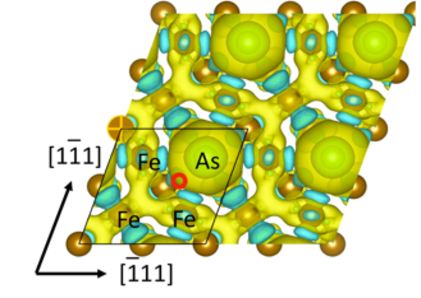
\includegraphics[width=0.45\linewidth]{Chap3/Fig9a.pdf}}\label{Chap:Mg_H:fig:9a}
  \subfigure[]{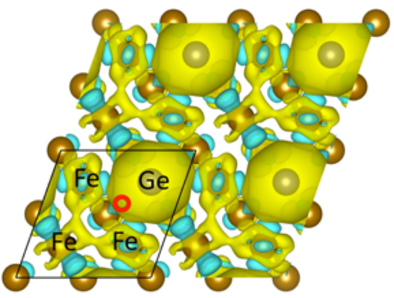
\includegraphics[width=0.45\linewidth]{Chap3/Fig9b.pdf}}\label{Chap:Mg_H:fig:9b}
  \\
  \subfigure[]{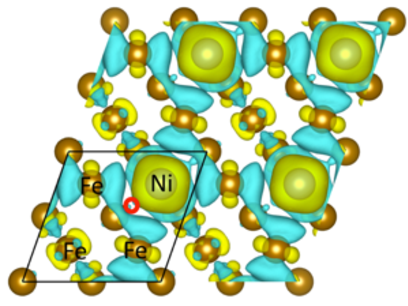
\includegraphics[width=0.45\linewidth]{Chap3/Fig9c.pdf}}\label{Chap:Mg_H:fig:9c}
  \subfigure[]{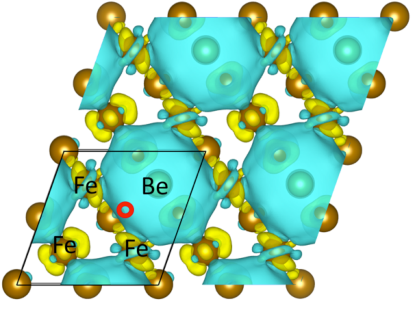
\includegraphics[width=0.45\linewidth]{Chap3/Fig9d.pdf}}\label{Chap:Mg_H:fig:9d}  
\caption[Top-down views of isosurfaces of electron density difference for (2x2) Fe (110) with one substitutional alloying atom in top surface layer]{Top-down views of isosurfaces of electron density difference ($\Delta \rho$ defined in Eq. \ref{Chap:Mg_H:eq:chargediff}) for (2x2) Fe (110) with one substitutional alloying atom in top surface layer. Surface Fe and alloy element X (X as As, Ge. Ni and Be in (a), (b), (c) and (d), respectively) are denoted. The open red circle is located at a hollow site I (Fig. \ref{Chap:Mg_H:fig:3b}) for hydrogen adsorption. The black box indicates the periodicity of a (2x2) Fe (110). The yellowish isosurface is $1.5x10^{-3}\frac{e}{bohr^3}$ corresponding to positive $\Delta \rho$ or electron accumulation after the substitutional alloying. The blue isosurface is $-1.5x10^{-3}\frac{e}{bohr^3}$ corresponding to negative $\Delta \rho$ or electron depletion after the substitutional alloying.}
  \label{Chap:Mg_H:fig9}
\end{figure}
\endgroup

\section{Electronic Mechanism of Mg Corrosion Inhibition}

In general, chemisorption on a transition metal surface is determined by two factors: a potential attractive energy term ($E_{attractive}$) related to the d-band center location relative to the Fermi level (i.e. so-called d-band center model), and a repulsive energy term ($E_{repulsive}$) related to the orbital overlap between the adsorbate orbital and the orbitals of other surface atoms (so-called Pauli repulsion) \cite{hammer1995electronic,hammer1995gold}:
\begin{align}
 %(9)
E_{chem adsorption} \sim E_{attractive} + E_{repulsive}
\label{Chap:Mg_H:eq:electronic}
\end{align}

We found that the effect of each of the 6 p-block elements identified as Mg corrosion inhibitors in Section 3c is negligible on the d-band center of Fe surface atoms. This was confirmed by computing and examining electronic density-of-states (Section S1 of the Supplementary Materials). Specifically, when one Fe atom in the top surface layer of (2x2) Fe (100) or (110) was substituted by an alloying atom from one of 6 p-block elements, the change of d-band center for all atoms in the top surface layer was always less than 0.2 eV. According to previous DFT studies of a series of transition metals, a change of $\sim$1 eV in the d-band center of their surface atoms results in a change of $\sim$0.5 eV in H adsorption energy \cite{greeley2006computational}. Thus, it is not expected that such small changes in the d-band center for an Fe surface with p-block substitutional elements reported here can induce significant variations of hydrogen adsorption strengths.

\begingroup
\begin{figure}[!ht]
  \centering
  \subfigure[]{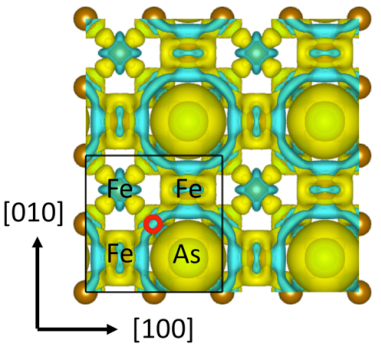
\includegraphics[width=0.45\linewidth]{Chap3/Fig10a.pdf}}\label{Chap:Mg_H:fig:10a}
  \subfigure[]{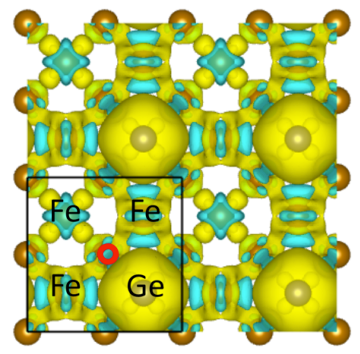
\includegraphics[width=0.45\linewidth]{Chap3/Fig10b.pdf}}\label{Chap:Mg_H:fig:10b}
  \\
  \subfigure[]{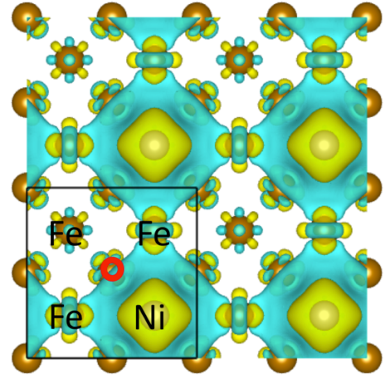
\includegraphics[width=0.45\linewidth]{Chap3/Fig10c.pdf}}\label{Chap:Mg_H:fig:10c}
  \subfigure[]{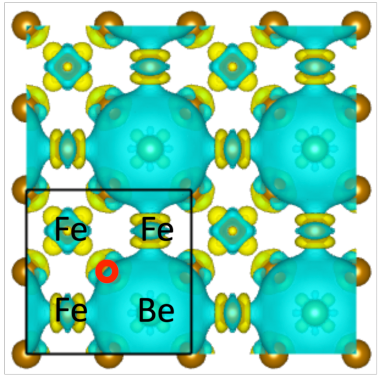
\includegraphics[width=0.45\linewidth]{Chap3/Fig10d.pdf}}\label{Chap:Mg_H:fig:10d}  
\caption[Top-down views of isosurfaces of electron density difference for (2x2) Fe (100) with one substitutional alloying atom in top surface layer]{Top-down views of isosurfaces of electron density difference ($\Delta \rho$ defined in Eq. \ref{Chap:Mg_H:eq:chargediff}) for (2x2) Fe (100) with one substitutional alloying atom in top surface layer. Surface Fe and alloy element X (X as As, Ge. Ni and Be in (a), (b), (c) and (d), respectively) are denoted. The open red circle is located at a hollow site I (Fig. \ref{Chap:Mg_H:fig:3b}) for hydrogen adsorption. The black box indicates the periodicity of a (2x2) Fe (100). The yellowish isosurface is $1.0x10^{-3}\frac{e}{bohr^3}$ corresponding to positive $\Delta \rho$ or electron accumulation after the substitutional alloying. The blue isosurface is $-1.0x10^{-3}\frac{e}{bohr^3}$ corresponding to negative $\Delta \rho$ or electron depletion after the substitutional alloying.}
  \label{Chap:Mg_H:fig10}
\end{figure}
\endgroup

We next examined surface charge redistribution by computing and displaying the difference, $\Delta \rho$, between the electron density of a pure (2x2) Fe (100)/(110) surface, $\rho_{Fe}$, and the electron density of the same surface unit cell with a substitutional X atom in the top surface layer, $\rho_{Fe+X}$, via
\begin{align}
 %(10)
\Delta \rho = \rho_{Fe+ X} - \rho_{Fe}
\label{Chap:Mg_H:eq:chargediff}
\end{align}
Results are shown in Figs. \ref{Chap:Mg_H:fig9} and \ref{Chap:Mg_H:fig10} for Fe (110) and Fe (100), respectively. Yellowish contours denote positive $\Delta \rho$ or regions of electron accumulation in the surface layer, while blue contours denote negative $\Delta \rho$ or electron depletion in the surface layer. Referring to Fig. \ref{Chap:Mg_H:fig:9a}, the yellowish contours surrounding the adsorbed As denote electron concentration in a shape resembling an s orbital with p-character. Fig. \ref{Chap:Mg_H:fig:9a} also shows a network of electron accumulation that encircles the As atom and flows through Fe surface atoms. This is somewhat counter-intuitive since As has five valence electrons, which is less than the eight in Fe. This electron accumulation around the As atom suggests the enhancement of both the spatial extent and electron density of the s/p orbital for the As atom compared with the pure Fe surface. When a H atom is absorbed at the hollow site near the As atom, indicated by the red circle in Fig. \ref{Chap:Mg_H:fig:9a}, the electrons from the adsorbed H atom and those from the substitutional As atom should overlap, and quantum mechanics requires that they must be orthogonal to each other. This drives up the energy and leads to so-called Pauli repulsion as described by $E_{repulsive}$ in Eq. \ref{Chap:Mg_H:eq:electronic}. Therefore, the s/p orbital for an As atom adsorbed on Fe (110) results in larger Pauli repulsion of the nearby H atom, making the H adsorption energy weaker relative to adsorption on a pure Fe surface. 

Similar effects were also predicted for adsorbed Ge on Fe (110), as shown in Fig. \ref{Chap:Mg_H:fig:9b}, as well as Al, Si, Ga, and P ($\Delta \rho$ contours not shown). Alternatively, the electron distribution is depleted around the adsorbed Ni atom in Fig. \ref{Chap:Mg_H:fig:9c} (relative to As in Fig. \ref{Chap:Mg_H:fig:9a}) and even more so around the adsorbed Be atom in Fig. \ref{Chap:Mg_H:fig:9d}. This is consistent with the observation from our high-throughput computations that neither Ni nor Be repels an H adsorbate on Fe surfaces, and the H adsorption energy in both cases is close to that of pure Fe (110). Observations for alloying elements on Fe (110) also apply to Fe (100) as shown in Fig. \ref{Chap:Mg_H:fig:10a} for As and Fig. \ref{Chap:Mg_H:fig:10b} for Ge (as well as Al, whose $\Delta \rho$ contours not shown). All of these elements have electron accumulation that resembles that for As on Fe (110) in Fig. \ref{Chap:Mg_H:fig:9a}, and their corresponding H adsorption energies notably change from -0.4 eV/atom to $\sim$ -0.2 eV/atom. Alternatively, Fig. \ref{Chap:Mg_H:fig:10c} shows that Ni has only a small local electron accumulation in Fe (100) while electron density is severely depleted around Be in Fig. \ref{Chap:Mg_H:fig:10d}. This is consistent with the conclusion from our high-throughput computations that H adsorption in the presence of Be and Ni on Fe (100) is not weakened.

\begingroup
\begin{figure}[!ht]
  \centering
  \subfigure[]{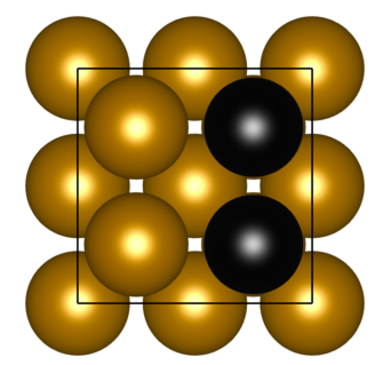
\includegraphics[width=0.45\linewidth]{Chap3/Fig11a.pdf}}\label{Chap:Mg_H:fig:11a}
  \subfigure[]{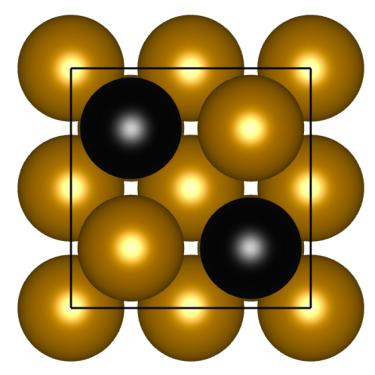
\includegraphics[width=0.45\linewidth]{Chap3/Fig11b.pdf}}\label{Chap:Mg_H:fig:11b}
  \\
  \subfigure[]{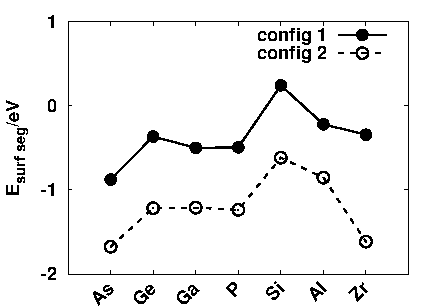
\includegraphics[width=0.45\linewidth]{Chap3/Fig11c.pdf}}\label{Chap:Mg_H:fig:11c}
  \subfigure[]{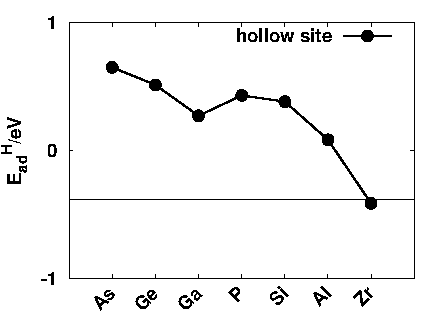
\includegraphics[width=0.45\linewidth]{Chap3/Fig11d.pdf}}\label{Chap:Mg_H:fig:11d}  
\caption[Effects of 6 p-block elements on higher surface alloying coverage]{(a) and (b): two different configurations ((a) as “config 1” and (b) as “config 2”)) for (2x2) Fe (100) with two atoms of a generic alloying element substituting two Fe atoms in the top surface layer. (c) Segregation energies $E_{surf seg}$ defined in Eq. (7) for the second substitutional alloying atom in (2x2) Fe (100) with two substitutional atoms in different final configurations ((a) and (b)). (d) H adsorption energies $E_{ad}^H$ defined in Eq. (8) on (2x2) Fe (100) with two substitutional alloying atoms in the top surface layer as “config 2” shown in (b).}
  \label{Chap:Mg_H:fig11}
\end{figure}
\endgroup

\section{Sensitivity Analysis for H Adsorption Energy on Surface Alloying Coverage}

All of the above evaluations are based on the three criteria in Section 2.1 with relatively simple but well-defined Fe surface structures with alloying elements. However, the quantitative predictions of alloying effects to Mg corrosion resistance require the accurate descriptions of surface and bulk structures of Fe-rich particles. As shown in Fig. \ref{Chap:Mg_H:fig:1b}, the overall alloying effect to reduce the \ac{HER} rate depends on the hydrogen adsorption energies, which can change when the substitutional alloying concentrations vary. However, the highly negative segregation energies $E_{surf}$ seg for these six candidates calculated using one substitutional alloying atom in a (2x2) surface unit cell shown in Figs. \ref{Chap:Mg_H:fig6} and \ref{Chap:Mg_H:fig7} suggest that there are substantial thermodynamic tendencies to have higher alloying element coverage on Fe surfaces. In addition, the reductions of hydrogen adsorption energies on Fe (100) surfaces due to $\frac{1}{4}$ \ac{ML} alloy surface coverage for the six alloying candidates are not very large (0.2 $\sim$ 0.4 eV per H atom), so the values of $E_{ad}^H$  on these alloyed surfaces are still close to the region corresponding to the maximum exchange current density of HER indicated by Fig. \ref{Chap:Mg_H:fig:1b}. These $E_{ad}^H$ values cannot strongly support the argument that such alloying elements can significantly reduce HER rates on Fe surfaces and inhibit the corrosion reactions on Mg alloys. For these reasons, we investigated the effects of higher substitutional alloying concentrations in the top layer of the two Fe surfaces. 

We first investigated whether it is possible to add a second substitutional alloying element in the top surface layer that already has one substitutional alloying element for a (2x2) Fe surface slab. Thus, we calculated the surface segregation energy $E_{surf}$ seg defined in Eq. \ref{Chap:Mg_H:eq:surf_seg} for the second substitutional alloying element in the top layer of (2x2) Fe (100) and (110) surface slabs, where $E_{surf}$ seg for the first alloying element already has strong negative values as shown in Figs. \ref{Chap:Mg_H:fig6} and \ref{Chap:Mg_H:fig7}. In Eq. \ref{Chap:Mg_H:eq:surf_seg}, $E_{bulk}$ is the energy of (2x2) surface slabs with one substitutional alloying element in the top surface layer and the other in the bulk far from the surface; $E_{surf}$ is the energy of a (2x2) surface slab with two substitutional alloying elements in the top surface layer. As shown in Figs. \ref{Chap:Mg_H:fig:11a} and \ref{Chap:Mg_H:fig:11b}, there are two possible configurations of two substitutional alloying elements in a (2x2) Fe (100) surface slab. As shown in Fig. \ref{Chap:Mg_H:fig:11c}, the alloying configuration in Fig. \ref{Chap:Mg_H:fig:11b} (“config 2”) always generates more negative $E_{surf}$ seg for the second substitutional element compared with their counterparts in Fig. \ref{Chap:Mg_H:fig:11a} (“config 1”). Thus, it is energetically favorable for these elements to have the configuration shown in Fig. \ref{Chap:Mg_H:fig:11b}. 

On these (2x2) Fe (100) surfaces, with two substitutional alloying elements in the top layer, there is at least one alloying element as the nearest neighbor for H atoms absorbed at all the hollow sites and bridge sites. Thus, the hydrogen adsorption energy should be very weak. The hydrogen adsorption energies on the hollow site in Fig. \ref{Chap:Mg_H:fig:11b}, the most favorable adsorption site on Fe (100), are indeed found to have very weak adsorption energy for the six p-block alloying element candidates. As shown in Fig. \ref{Chap:Mg_H:fig:11d}, $E_{ad}^H$ of As, Ge, Ga, P, Si and Al are positive values, with weaker hydrogen adsorption than that on the noble metal (Au, Ag) surfaces considered in Fig. \ref{Chap:Mg_H:fig:1b}. Such significant reductions of hydrogen adsorption energies suggest that the Volmer reaction in Eq. \ref{Chap:Mg_H:eq:Tafel} is indeed slow enough to impede the \ac{HER} rate on cathode sites. Alternatively, the (2x2) Fe (100) surface with 2 substitutional Zr atoms still has H adsorption energies comparable to those on pure Fe surfaces, suggesting higher surface concentrations of Zr (possibly for other similar transition metal elements like Hf) cannot result in noticeable changes in \ac{HER} rates. Similar results apply to alloying of Fe (110) surfaces.

The above DFT calculations suggest that one-half of a \ac{ML} of alloying element X (As, Ge, Ga, etc.) can effectively inhibit the HER on Fe surfaces. Usually, the concentration of Fe impurities in Mg alloys is of the order of 100 ppm. Here, we assume all Fe impurities exist as second-phase particles in a nano-cube shape and each cube has 6 {100} facets each with a length L = 10 or 100 nm to a side. A simple analysis shows that $\sim$10 ppm or $\sim$1 ppm of alloying element X is enough to cover one-half of all Fe second-phase particle surfaces. Our calculations suggest that these alloying elements have a strong preference to segregate to Fe surfaces compared with the Mg or the Fe bulk lattice according to our DFT results, we conclude that $\sim$10 ppm level of these alloying elements will be sufficient to show a noticeable effect on Mg corrosion resistance if there are no other phases/locations that can strongly attract these alloying elements. In reality, other stable occupation sites for these alloying elements could be on different precipitate phases and grain boundaries, so a higher concentration of alloying element X may be required to significantly enhance corrosion resistance of Mg alloys.

\section{Generalization on Other Precipitates}

Finally, it is well known that Mg may contain other phases that can function as cathodic sites in Mg corrosion. Examples are the $\beta$-phase, Mg17Al12 \cite{guo2017influence}, Cu \cite{kawabata2012influence} and Ni \cite{hanawalt1942corrosion}. In fact, Song and Artens \cite{song2003understanding} claim that of the three types of second-phase particles that are rich in Ni, Fe and Cu, respectively, Ni is the most detrimental with Fe intermediate to Ni and Cu. Thus, the high-throughput computational strategy was applied to Cu and Ni particles cases by again following the three criteria in Section 2.1 to investigate whether the 6 p-block elements can inhibit HER on surfaces of these second-phase particles. 

\begingroup
\begin{figure}[!ht]
  \centering
  \subfigure[]{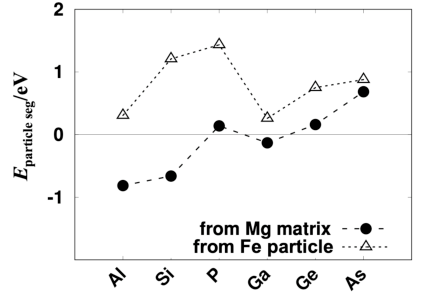
\includegraphics[width=0.45\linewidth]{Chap3/Fig12a.pdf}}\label{Chap:Mg_H:fig:12a}
  \subfigure[]{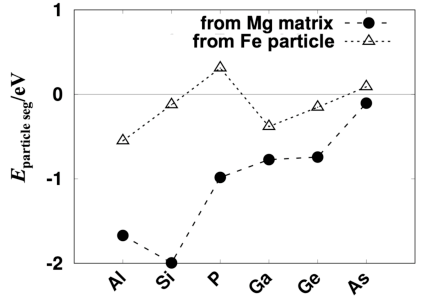
\includegraphics[width=0.45\linewidth]{Chap3/Fig12b.pdf}}\label{Chap:Mg_H:fig:12b}
  \\
  \subfigure[]{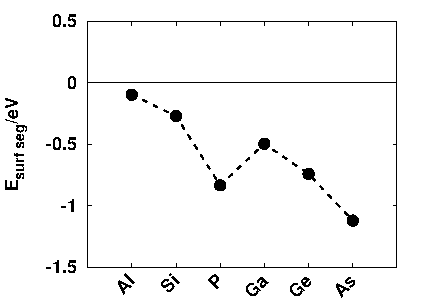
\includegraphics[width=0.45\linewidth]{Chap3/Fig12c.pdf}}\label{Chap:Mg_H:fig:12c}
  \subfigure[]{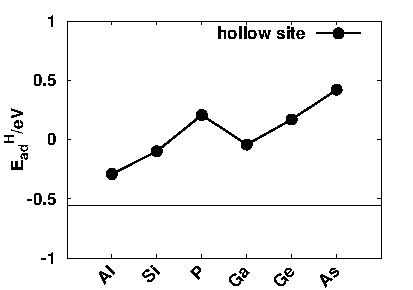
\includegraphics[width=0.45\linewidth]{Chap3/Fig12d.pdf}}\label{Chap:Mg_H:fig:12d}  
\caption[Effects of 6 p-block elements on other precipitates(Cu and Ni)]{(a) and (b): Bulk segregation energies $E_{particle seg}$ for 6 p-block alloying elements in bulk Cu (a) and Ni (b) second-phase particles in Mg matrix, respectively. The solid circles denote the segregation energies of alloying elements in bulk Cu/Ni particles over bulk Mg matrix, and the open triangles denote the segregation energies of alloying elements in bulk Cu/Ni particles over bulk Fe particles. The energy differences are defined in equations similar to Eq. \ref{Chap:Mg_H:eq:particle_seg}. Preference for a bulk Cu/Ni particle over the bulk Mg/Fe particles requires that an alloying element should have a significantly negative value of $E_{particle seg}$. (c) Surface segregation energies $E_{surf seg}$ defined in Eq. \ref{Chap:Mg_H:eq:surf_seg} for Ni (111) of 6 p-block alloying elements. A qualified alloy candidate should have a strongly negative value of Esurf seg. (d) H adsorption energies $E_{ad}^H$, which is defined in Eq. \ref{Chap:Mg_H:eq:H_ads}, on (2x2) Ni (111) surfaces with $\frac{1}{4}$ \ac{ML} alloying atom in the top surface layer. The horizontal line stands for the H adsorption energy of pure Ni (111) surface hollow site.}
  \label{Chap:Mg_H:fig12}
\end{figure}
\endgroup

For the first criterion, we calculated the alloy segregation energy in the bulk of Cu and Ni particles when the alloying element X comes from the Mg matrix or bulk Fe particles via following Eq. \ref{Chap:Mg_H:eq:particle_seg}. For Cu, only Al and Si have a strong energetic preference (more negative than -0.5 eV) to stay in bulk Cu particles compared to bulk Mg as shown by closed black circles in Fig. \ref{Chap:Mg_H:fig:12a}. The segregation energies for P, Ga or Ge are between $\pm$0.1 eV, and As even has a strong segregation (over +0.5eV) in Mg bulk matrix relative to bulk Cu particles.  Therefore, As, Ge, Ga or P does not have a strong preference to be stable in Cu bulk. In addition, all the six p-block elements show thermodynamic preferences for bulk Fe particles over bulk Cu particles as shown by the open triangles in Fig. \ref{Chap:Mg_H:fig:12a}. Alternatively, Fig. \ref{Chap:Mg_H:fig:12b} suggests that each of the six elements have a thermodynamic preference to stay in bulk Ni particles compared to the bulk Mg matrix, and all of these elements do not show a strong thermodynamic preference for bulk Fe particles over bulk Ni particles. Therefore, the ability of the six p-block alloying elements to inhibit HER on Cu particles is limited and out of the scope of further discussions, and we will only focus on Ni.

For the second criterion, the surface segregation energies of the six elements were calculated via Eq. \ref{Chap:Mg_H:eq:surf_seg}, which shows that all the six elements are also more stable on the clean Ni(111) surface compared to Ni bulk according to Fig. \ref{Chap:Mg_H:fig:12c}. For the calculations of H adsorption energies $E_{ad}^H$, defined in Eq. \ref{Chap:Mg_H:eq:H_ads}, H adsorption energies at the FCC hollow site on Ni(111) surfaces were investigated by only allowing H and surface atoms to relax in the direction normal to the Ni(111) surface, following what was done for Fe (110) as described in Section 3c. Similar to their effects on the surfaces of Fe second-phase particle, all six p-block elements weaken H adsorption energies on Ni (111) surfaces as shown in Fig. \ref{Chap:Mg_H:fig:12d}. On (2x2) pure Ni (111) surfaces, the H adsorption energy is -0.56 eV for $\frac{1}{4}$ ML H coverage. Among the six elements, As, P and Ge alloyed surfaces show very weak H adsorption energies (to +0.42, +0.21 and +0.17 eV, respectively, comparable to $E_{ad}^H$ on the noble metal (Au, Ag) surfaces in Fig. \ref{Chap:Mg_H:fig:1b}). Germanium, Si, and Al can moderately weaken H adsorption energies (to -0.04, -0.10 and -0.29 eV). Hence, the six p-block elements that are effective on the two Fe surfaces are also effective on Ni(111).

\section{Conclusions}

A strategy for increasing the corrosion resistance of Mg with Fe impurities that has gained significant traction in the experimental literature involves finding alloying elements that slow down or even inhibit the HER as the cathodic corrosion reaction on surfaces of Fe second-phase particles. The present study used a high-throughput DFT calculation strategy to search for such alloying elements based on three criteria. First, an element must show a thermodynamic preference for bulk BCC Fe over bulk HCP Mg; second, an element must be thermodynamically more stable on Fe (100) and Fe (110) than bulk Fe; third, the H adsorption energies on both Fe (100) and Fe (110) with an alloying element in their topmost layers should be significantly reduced or enhanced relative to the adsorption energies of a lone H atom on pure Fe (100) and (110), suggesting likely interference with the HER rate. The major conclusions from this study are as follows:

 (1) Calculations show that As as an alloying element can satisfy the above three criteria. Depending on the As surface concentration, the hydrogen adsorption energies can be significantly reduced ($>$ $\sim$10 $k_{B}T$ at the room temperature T $\sim$ 300 K), which can slow down the generation of adsorbed H atoms through water molecule dissociation (the Volmer reaction, Eq. \ref{Chap:Mg_H:eq:Volmer}) in the HER reaction mechanisms. This is different than previous arguments where As can slow down the hydrogen recombination on Fe surfaces. The extent to which H adsorption energies are reduced depends on As concentration in the top surface layer of Fe. If one-half of the Fe atoms are substituted by As atoms in the top layer, which is thermodynamically favorable compared with As atoms in Fe bulk, then the H adsorption strength on such surface is predicted to reduced by $\sim$1 eV per H atom, even weaker than H adsorption strength on Au surfaces, which is extremely inactive for HER.
 
(2) Of the 68 potential elements considered as possible corrosion inhibitors, the following six elements, rank ordered by their ability to reduce (or destabilize) H adsorption on Fe surfaces, meet all three criteria: $\text{As} > \text{Ge} > \text{Si} > \text{Ga} > \text{P} \approx \text{Al}$. Each of the six identified elements likely inhibit the Volmer reaction \ref{Chap:Mg_H:eq:Volmer} necessary for the HER on Fe impurities that function as cathode surfaces. Identification of As and Ge as the best of all 68 elements examined is in qualitative accord experiments These p-block elements are also found to have the potential to reduce \ac{HER} on Ni second-phase particles according to the same criteria. However, the ability of these p-block alloying elements to inhibit \ac{HER} on Cu second-phase particles is limited because these elements do not show strong preferences to be stable in Cu particles relative to those in Mg matrix.

(3) Electron density difference contours show that excess electrons accumulate in the outer-shells (e.g. s and p orbitals) of each atom of the six elements replacing a Fe atom in both Fe (100) and Fe (110). This causes an enhancement to Pauli repulsion between an adsorbed H atom at an adjacent surface site and a substitutional alloying atom when orbitals of the latter overlap with the s-orbital of an H adsorbate. A significant reduction of H adsorption energy results (or destabilization of H binding) by increasing the repulsion. 
